\documentclass[a4paper,11pt]{article}

\usepackage{../préambule}

\newgeometry{top=1cm,bottom=1cm,left=1cm,right=1cm}

\makeatletter
\renewcommand{\maketitle}{%
{\scriptsize colle dans ton cahier d'exercices}
	\begin{center}
		\LARGE
		\myuline{\@title}
		\vspace{0.5em}
	\end{center}
}
\makeatother

\title{Utilisation du tableur}
\author{}
\date{}

\begin{document}

\maketitle

\begin{center}
	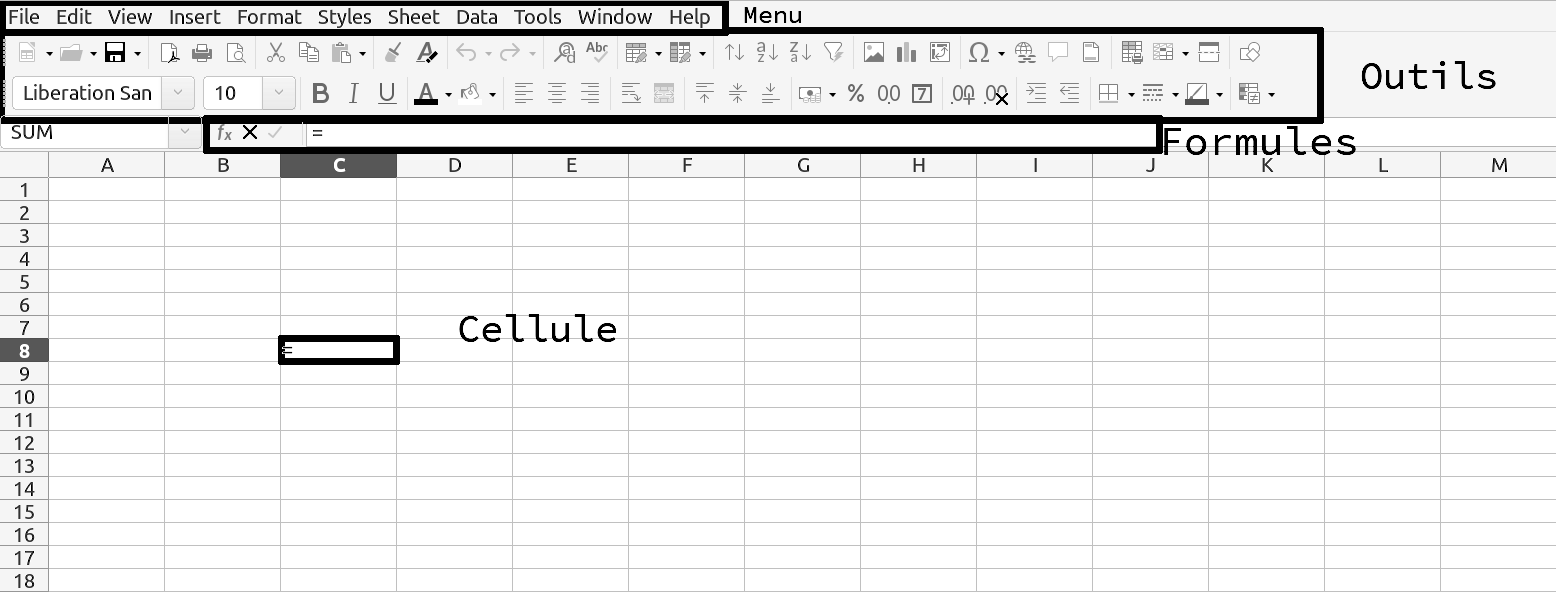
\includegraphics[width=0.8\textwidth]{Images/[gray] Introduction tableur - tableur windows.png}
\end{center}

\begin{exercice}\
	\begin{enumerate}
		\item Fait, sans calculatrice, les calculs suivants:
		      \begin{itemize}
			      \item $50 × 31 = $ ...... % 1550
			      \item $2,3 × 7,9 = $ ........ % 18,17
			      \item $8,16 + 9,87 = $ ........ % 18,03
		      \end{itemize}
		\item Connecte-toi sur \url{laclasse.com}, va dans \faicon{briefcase} \textbf{docs}, et \squared{\faicon{download} télécharge} le fichier \textbf{Mathématiques → Séance tableur 1 → fiche-de-calcul}. Ouvre ensuite ce fichier, et observe ce qu'il y a dedans. \vspace{1em}

		      Utilise le tableur pour vérifier tes résultats.
		\item En utilisant le tableur, effectue les calculs suivants, et note les résultats :
		      \begin{itemize}
			      \item $(346 × 78) + (346 + 78) = $ ........
			      \item $5,8 + (5,8 × 45,7) = $ ........
			      \item $(57,3 × 5,6) + (57,3 + 5,6) = $ ........
			      \item $(78,8 × 89,7) + 78,8 = $ ........
		      \end{itemize}
		\item Clique sur la cellule \squared{C2}, et regarde la zone de \textbf{Formules}. Il y a normalement écrit \squared{=A2*B2}.

		      Remplace ce texte par \squared{=2*B2}, puis appuie sur \textit{Entrée}. Qu'observes-tu ?

		      En utilisant le tableur, effectue les calculs suivants :
		      \begin{itemize}
			      \item $67 × (56 + 67) = $ ......

			      \item $9,8 × (34 + 9,8) = $ ......

			      \item $596 × (5,9 + 596) = $ ......
		      \end{itemize}
	\end{enumerate}
\end{exercice}

\begin{exercice}\
	\begin{enumerate}
		\item Remplis la colonne \textbf{A} avec les nombres suivants : $6$,\hspace{0.5em} $8$,\hspace{0.5em} $9,6$,\hspace{0.5em} $12,8$ et $14,36$ (cellules A2 à A6).
		\item \begin{itemize}
			      \item Sélectionne la cellule A7.
			      \item Dans la zone de formules, clique sur le symbole “$Σ$”, juste à gauche du signe “=”.
			      \item Sélectionne “Somme”, et appuie sur \textit{Entrée}.
		      \end{itemize}
		      Quel est le nombre dans la cellule A7 ? ........
		\item Calcule $6 + 8 + 9,6 + 12,8 + 14,36$ : ......
		\item Remplis la colonne \textbf{B} avec les nombres suivants : $2,1$,\hspace{0.5em} $0,8$,\hspace{0.5em} $10$,\hspace{0.5em} $3$ et $1,6$ (cellules B2 à B6).
		\item Sélectionne la cellule $C2$. Passes ta souris sur le bord inférieur droit de cette cellule : vois-tu quelque chose de spécial ?

		      \textbf{Clique sur ta souris et maintiens}, puis bouge ta souris vers le bas. Qu'observes-tu ?
		\item Sans changer d'autres choses dans le tableur, trouve le résultat de $14,36 × 1,6$ : ........
	\end{enumerate}
\end{exercice}

\end{document}